\chapter{Probleemstelling}
Om tot het idee van dit project te komen hebben we eerst bestaande locatie-gebaseerde toepassingen en online marketing tools geanalyseerd. Vervolgens hebben we beide concepten gecombineerd in één applicatie, nl. Triump.

Vandaag bestaan reeds verschillende locatie-gebaseerde applicaties waarmee gebruikers hun huidige locatie kunnen delen met hun vrienden. 
De bekendste voorbeelden hiervan zijn Foursquare\cite{foursquare} en Swarm\cite{swarm}.
Foursquare is een sociale netwerksite die gebruikers plaatsen laat categoriseren en beoordelen.
Het is een mobiele applicatie waarmee men hippe locaties met elkaar kan delen. Met Swarm daarentegen kunnen gebruikers `inchecken' op plaatsen en hun locatie delen met andere gebruikers. Swarm is een mobiele applicatie, die gebruik maakt van de Foursquare's locatiedatabase. Swarm is eerder gericht op het delen van locatieupdates in plaats van ervaringen en tips zoals het geval bij Foursquare.
Hoewel Swarm en Foursquare beide gericht zijn op het sociaal gebeuren, wordt er geen nadruk gelegd op het `samenbrengen' van mensen. 

Daarnaast onderzochten we ook online marketing platformen. Momenteel gebeurt online marketing voornamelijk op een manier die door gebruikers als intrusief en ongewenst ervaren wordt via online advertenties. Qustomer\cite{qustomer} daarentegen is een online marketing tool die erin is geslaagd om naast advertising ook iets extra aan gebruikers te bieden. Qustomer biedt gebruikers een klantenkaart in de vorm van een applicatie op de mobiele telefoon. Deze klantenkaart kan door verschillende ondernemingen gebruikt worden. Net zoals bij traditionele klantenkaarten, kan een gebruiker punten opsparen en hiermee promoties verkrijgen. Qustomer en andere van deze platformen staan los van enige vorm van sociale media, en bijgevolg is de aantrekkingskracht naar gebruikers toe eerder beperkt.

Vandaag bestaan beide media, locatie-gebaseerde sociale applicaties en online marketing tools, volledig onafhankelijk van elkaar en zijn er geen toepassingen die beide concepten combineren. 
Promoties vormen een stimulans om mensen gebruik te laten maken van de diensten van een bedrijf. Indien de promoties gericht zijn op groepen mensen en volgens het Groupon-principe werken, kunnen promoties een middel zijn om mensen samen te brengen.
In het Groupon-principe verkrijgt men namelijk voordelen door in grote groep diensten aan te kopen.
Afgelopen jaar Foursquare heeft 45 miljoen actieve gebruikers bereikt, en dat aantal is nog steeds aan het groeien. \cite{users}. Foursquare is dus een platform met het potentieel om een enorm publiek te bereiken wegens zijn functie als sociaal netwerk. 

Indien men concepten zoals Foursquare en Qustomer combineert, krijgt men een platform waarbij men mensen stimuleert om samen te komen omwille van promoties en men deze bereikt via Foursquare.
Triump is een mobiele applicatie met als doel beide te koppelen.
Concreet breidt Triump de functionaliteit van Foursquare uit en wordt het marketing aspect gebaseerd op het concept van Qustomer.
\begin{figure}[ht]
\begin{minipage}[b]{0.25\linewidth}
\centering
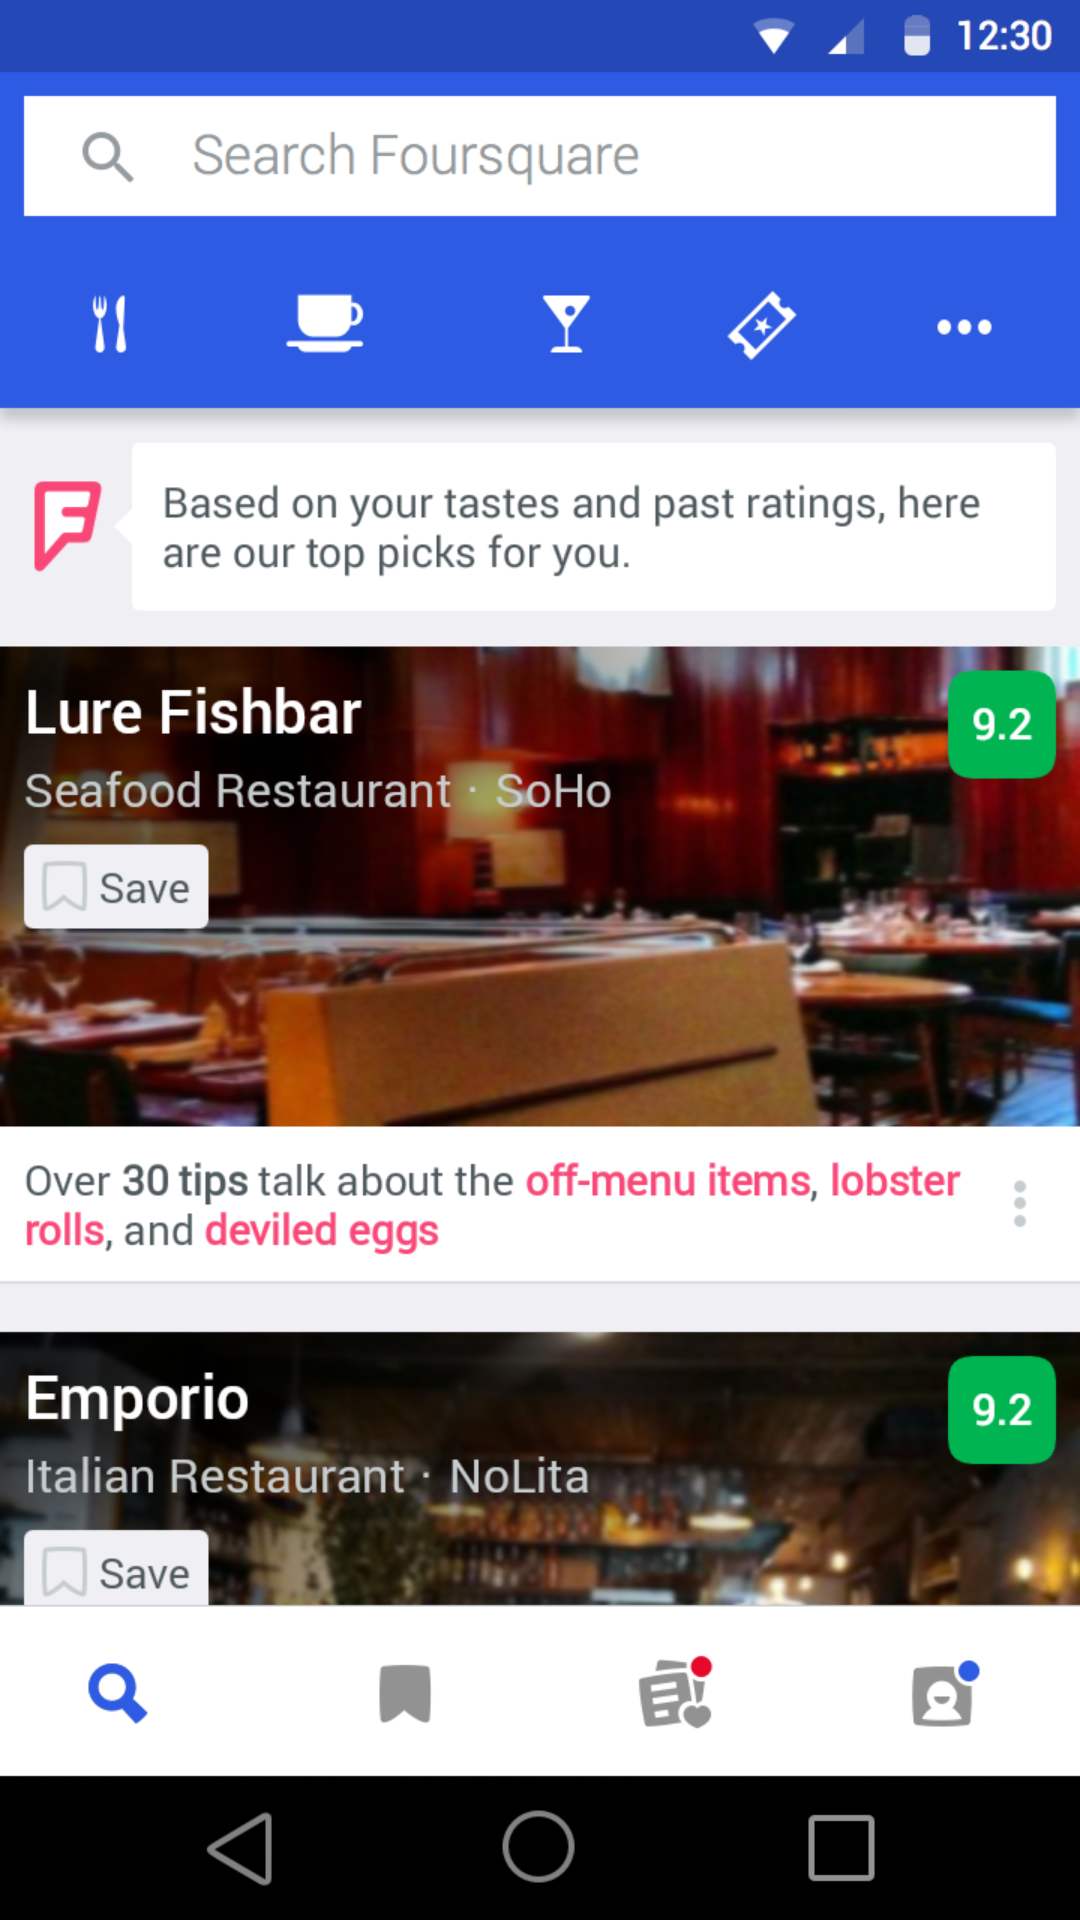
\includegraphics[width=\textwidth]{screenshot_foursquare}
\caption{Foursquare}
\label{fig:screenshot_foursquare}
\end{minipage}
\hspace{1.5cm}
\begin{minipage}[b]{0.25\linewidth}
\centering
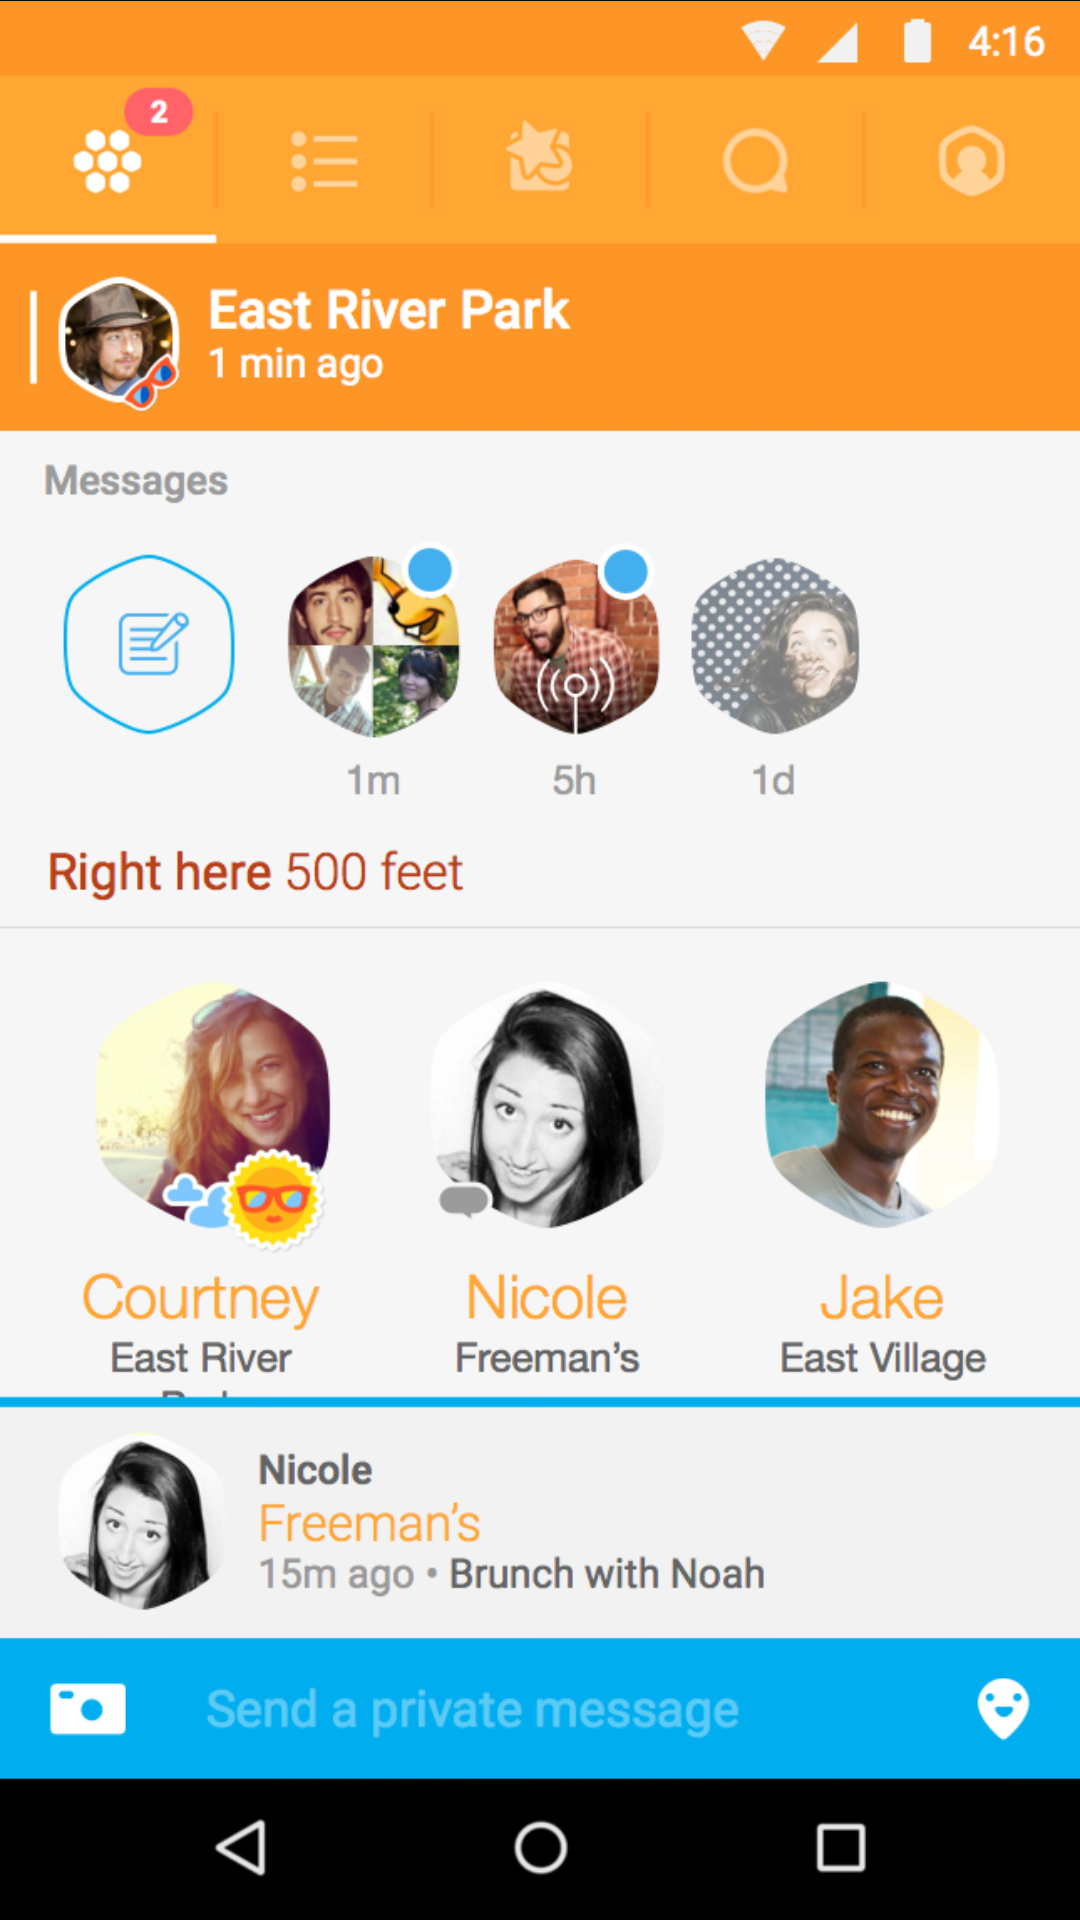
\includegraphics[width=\textwidth]{screenshot_swarm}
\caption{Swarm}
\label{fig:screenshot_swarm}
\end{minipage}
\hspace{1.5cm}
\begin{minipage}[b]{0.25\linewidth}
\centering
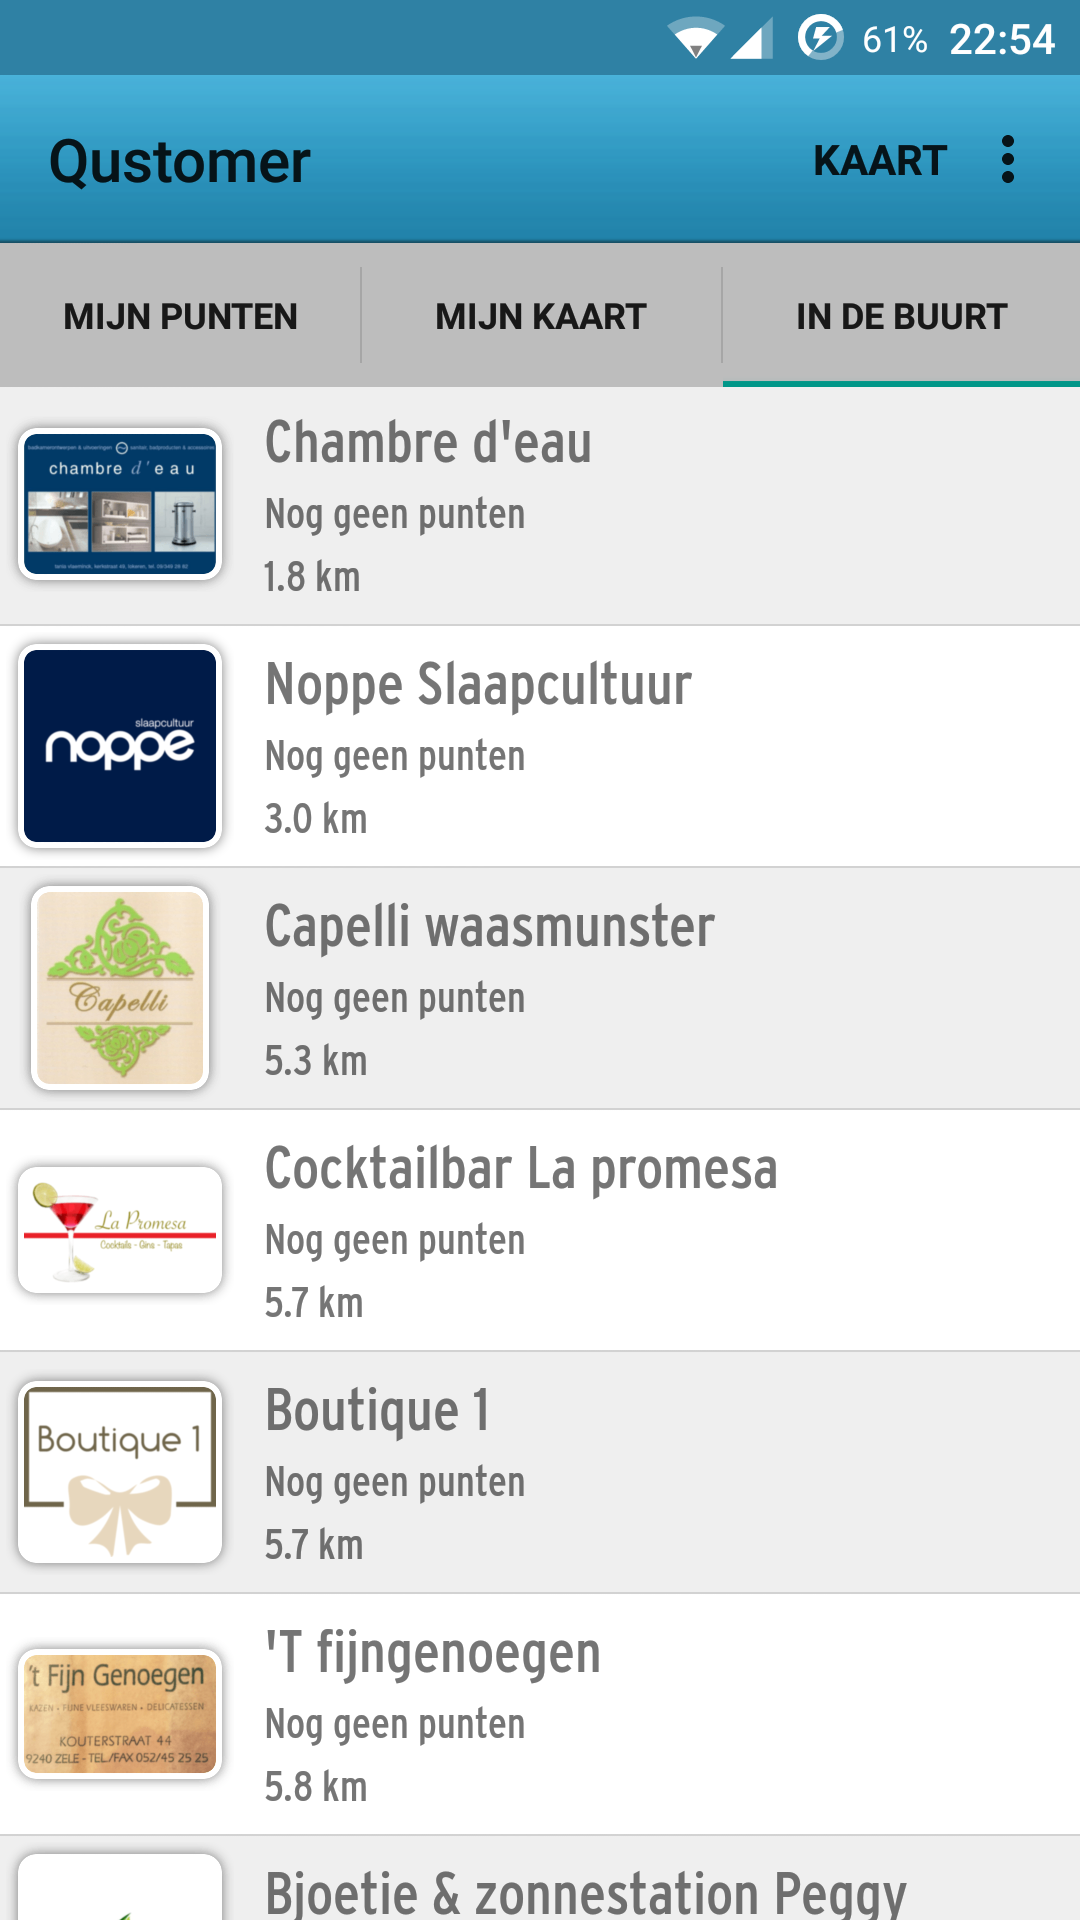
\includegraphics[width=\textwidth]{screenshot_qustomer}
\caption{Qustomer}
\label{fig:screenshot_qustomer}
\end{minipage}
\end{figure}

